% EmoViz Technical Report — documentation of the technical build (not assessed dissertation prose)
\documentclass[11pt,a4paper]{article}
\usepackage[margin=2.4cm]{geometry}
\usepackage{graphicx}
\usepackage{booktabs}
\usepackage{xcolor}
\usepackage{titlesec}
\usepackage{enumitem}
\usepackage[hidelinks]{hyperref}
\usepackage{helvet}
\usepackage{parskip}

\definecolor{ink}{HTML}{1D2227}
\definecolor{blue}{HTML}{31708F}
\definecolor{gold}{HTML}{B07D2B}
\definecolor{soft}{HTML}{5A636C}
\definecolor{green}{HTML}{3C7A4E}
\definecolor{red}{HTML}{9E3B33}

\titleformat{\section}{\Large\bfseries\color{ink}}{\thesection}{0.8em}{}
\titleformat{\subsection}{\large\bfseries\color{blue}}{\thesubsection}{0.7em}{}
\setlist{nosep, leftmargin=1.4em}

\newcommand{\pass}{\textcolor{green}{\textbf{PASS}}}
\newcommand{\finding}[1]{\textcolor{blue}{\textbf{#1}}}

\begin{document}

% ---------------- title ----------------
\begin{center}
{\huge\bfseries EmoViz: Technical Report}\\[6pt]
{\Large Visualising Emotion --- the complete analysis pipeline}\\[10pt]
{\color{soft} Technical documentation of the software, experiments and findings}\\[4pt]
{\color{soft} MSc Dissertation Project of Shre Hari Prem Anandh · Supervisor: Dr Chaona Chen}\\
{\color{soft} School of Computer Science, University of Sheffield · September 2026}\\[6pt]
{\small\color{soft}\emph{This document records the technical work; the assessed dissertation is written separately by the student.}}
\end{center}

\vspace{4pt}
\hrule
\vspace{10pt}

% ---------------- executive summary ----------------
\section*{Executive summary}
This project asks a question almost untouched in the text-to-image literature: \textbf{when an AI
turns words about a feeling into a picture, how far does an automatic reading of the picture agree
with an automatic reading of the words?} Working on a unique dataset of \textbf{1{,}025
prompt--drawing records} --- each rendered as a black-and-white line drawing by DALL·E at a public
engagement event --- we built, validated and verified a complete measurement pipeline. Five findings
emerged:

\begin{enumerate}
\item \textbf{Agreement is much higher where the describer reports a face.} Face-classified drawings
agree with the prompt reader on valence sign \textbf{73.9\%} of the time (family agreement 61.9\%);
scene-classified drawings \textbf{42.9\%} (family 35.6\%). Both exceed chance; the difference is
$+30.9$\,pp [$+22.6$, $+40.6$], clustered permutation $p = 0.0001$. The scene result weakens on
distinct prompts.
\item \textbf{The pipeline passes its specificity check.} For prompts the text reader labels neutral
(40\% of the data), valence--arousal agreement sits at its null (76.6\% vs 76.6\%, $z = +0.3$);
sign and family are degenerate there and carry no $z$.
\item \textbf{The same words do not reliably give the same reading.} Across 87 prompts drawn 2--42
times each, the image reader returns the same family for 68.8\% of drawings within a group against a
permutation null of 59.4\% ($z = +4.5$); 28 of 87 groups are fully consistent against 14.5 by chance.
\item \textbf{Method matters --- describe-then-extract agrees far more closely.} Like for like, the
describe-then-extract reader reaches 53.0\% family agreement against 22.4\% for asking CLIP directly
($+30.6$\,pp [$+25.5$, $+35.6$], cluster-level $p < 0.0001$).
\item \textbf{The reading rests on one word.} A template ablation (NLI stage only re-run) shows that
removing the describer's expression sentence collapses family agreement from 53.0\% to 20.3\%, the
other clauses move it 1--3\,pp, and under a people-aware template the scene reading falls to its
null (4.7\% vs 3.4\%, $z = +1.6$): faces, and only faces, for this reader.
\end{enumerate}

All results are measured against random-pairing null baselines with clustered-bootstrap 95\%
intervals, re-audited on 1 and 9 September 2026 with the corrections recorded below, checked on
deduplicated prompts, and covered by the automated self-test, whose numeric layer pins every headline
value to the result file that produces it.

% ---------------- dataset ----------------
\section{The dataset --- and how every record is used}
\begin{center}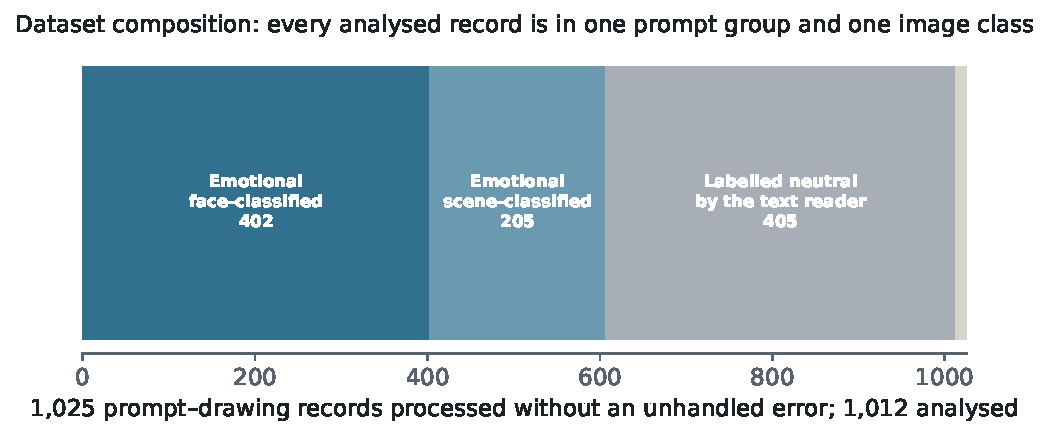
\includegraphics[width=0.98\textwidth]{../figures/fig5_dataset.pdf}\end{center}

1{,}025 text--image pairs from Festival of the Mind 2024 (Sheffield): visitors typed how they felt;
DALL·E drew each entry as monochrome line art. Median prompt length is 4 words; mixed feelings
(``tired but happy'') are common. Key data-engineering facts established:

\begin{itemize}
\item \textbf{Three incompatible filename schemes} and two lowercase extensions were unified by a
robust loader (\texttt{emoviz/data.py}) --- a na\"ive loader resolves under 20\% of files.
\item \textbf{Hidden provenance metadata} (C2PA) was recovered from inside every PNG, yielding
per-image timestamps that identified records 1--13 as \textbf{pre-festival developer tests}
(excluded from analysis; still processed).
\item \textbf{All 1{,}025 images processed with no unhandled errors}; every analysed record belongs to exactly one
prompt group (607 emotional / 405 labelled neutral) and one face/scene group (591/421) --- the splits are
groupings, not exclusions, and \emph{all} groups are reported.
\item 87 prompts repeat 2--42 times (336 records) --- used both as a natural consistency experiment
and for a deduplication robustness check.
\end{itemize}

% ---------------- architecture ----------------
\section{Pipeline architecture}
Following the supervisor's direction, the pipeline never asks a vision model for an emotion.
Instead it \emph{describes} then \emph{extracts}:

\begin{center}
\begin{tabular}{@{}lll@{}}
\toprule
\textbf{Stage} & \textbf{Component} & \textbf{Output}\\
\midrule
0 · Split & GoEmotions (prompts) / BLIP-VQA cues (images) & emotional?\ · face?\\
1 · Describe & \textbf{BLIP-VQA}: expression, action, posture, scene & neutral description\\
2 · Extract & \textbf{Zero-shot NLI} (facts $\rightarrow$ feeling), both sides & top-3 emotions\\
3 · Compare & \textbf{Similarity ladder}, not exact match & 4 metrics + null $z$\\
\bottomrule
\end{tabular}
\end{center}

The similarity ladder scores each pair at four granularities --- valence--arousal proximity,
valence sign, Ekman family, and probability-weighted top-3 overlap --- and every metric is
referenced to a \textbf{random-pairing null} (300 shuffles): every value is read as distance above
its own null.

\subsection{Engineering the pipeline: what was tried and rejected}
Each link was tested \emph{before} being trusted; the failures shaped the final design and are
findings in their own right:

\begin{center}
\begin{tabular}{@{}p{4.6cm}p{9.6cm}@{}}
\toprule
\textbf{Candidate} & \textbf{Why rejected (evidence)}\\
\midrule
GoEmotions on image descriptions & Collapses to \emph{neutral} 0.95+ --- it needs first-person feeling words; scene descriptions have none.\\
Single BLIP caption $\rightarrow$ NLI & Captions too terse (``a man with hands in the air'') --- NLI collapses to \emph{surprise}.\\
Qwen2.5-VL-3B describer & 7\,GB fp16 exceeded laptop RAM; thrashed into swap, zero progress in 4\,h\,45\,min. Machine supports only sub-1B describers.\\
Florence-2 describer & Incompatible with transformers 5.14 (\texttt{forced\_bos\_token\_id} failure in remote code).\\
\textbf{BLIP-VQA (chosen)} & $\sim$0.4B, native, $\sim$1.5\,s/record; its \emph{``what is the facial expression?''} answer supplies exactly the affective cue NLI needs.\\
\bottomrule
\end{tabular}
\end{center}

% ---------------- results ----------------
\section{Findings}

\subsection{Finding 1 --- agreement is much higher where the describer reports a face}
\begin{center}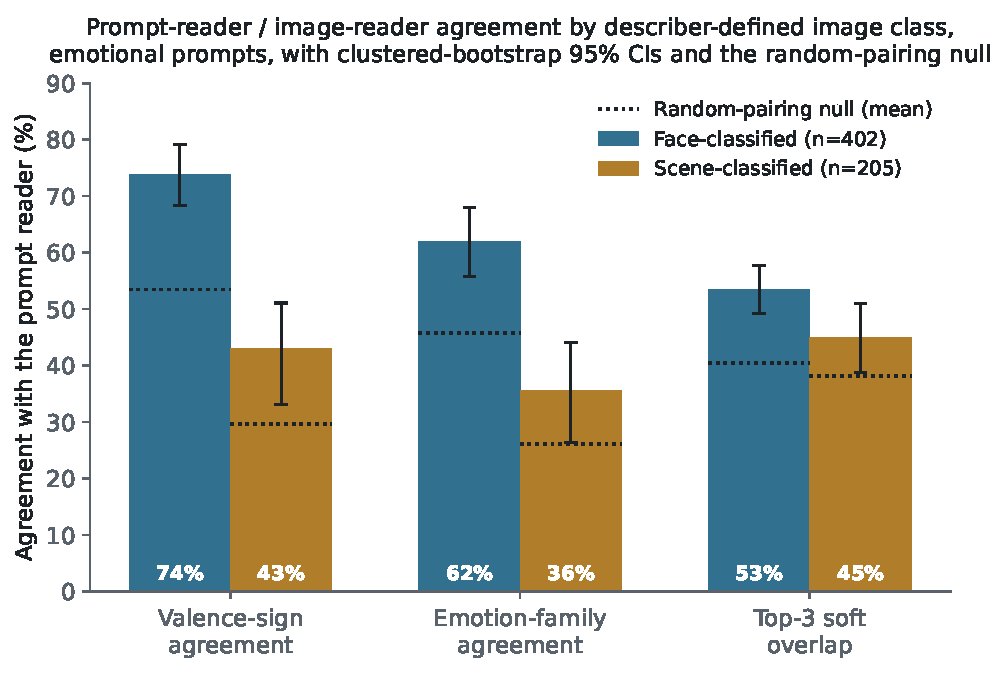
\includegraphics[width=0.9\textwidth]{../figures/fig1_face_vs_scene.pdf}\end{center}
Face-classified drawings (n=402) agree with the prompt reader on valence sign 73.9\% ($z\!=\!+10.4$;
95\% CI [68.3, 79.2]) vs 42.9\% for scene-classified (n=205, $z\!=\!+5.8$; [33.1, 51.1]); family
agreement 61.9\% vs 35.6\%. The difference is $+30.9$\,pp [$+22.6$, $+40.6$] (family $+26.3$\,pp
[$+18.4$, $+35.3$]), clustered permutation $p = 0.0001$. On distinct prompts the face result holds
($z\!=\!+8.4$) and the scene result weakens (valence sign $z\!=\!+3.5$, family $z\!=\!+2.6$).
\emph{Caveat (stated honestly):} the split is governed by the describer's people-count answer, and
the template asserts an expression for a drawing with no person (406 of the 414 no-people scene
records carry one), so the image-side reading for scenes is largely noise; the split is entangled
with the measure. Finding 5 makes this concrete: under a people-aware template the scene rows fall
to their null, so the contrast is faces, and only faces, for this reader.

\subsection{Finding 2 --- the specificity check passes}
\begin{center}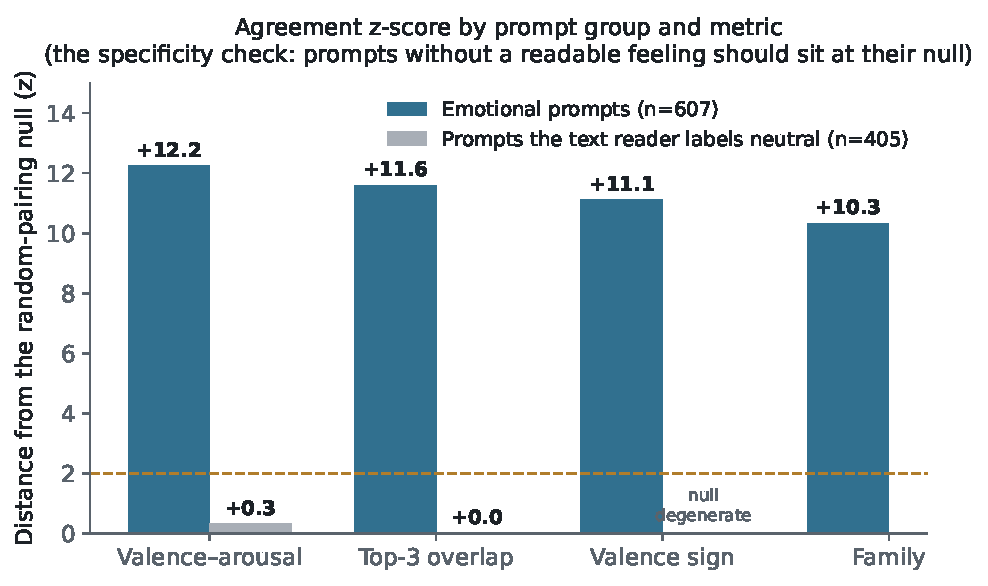
\includegraphics[width=0.72\textwidth]{../figures/fig3_z_by_prompt_group.pdf}\end{center}
Emotional prompts sit at $z\!\approx\!+12$ on valence--arousal; prompts the text reader labels
neutral (``pigs'', ``mickey mouse'') sit at $z\!=\!+0.3$ --- indistinguishable from chance. Only the
valence--arousal measure is informative on that subset (sign and family are degenerate by
construction); 68 of the 405 contain a plain affect word and two are a name alone, and the cleaned
335 give $z\!=\!+0.04$.

\subsection{Finding 3 --- the same words do not reliably give the same reading}
\begin{center}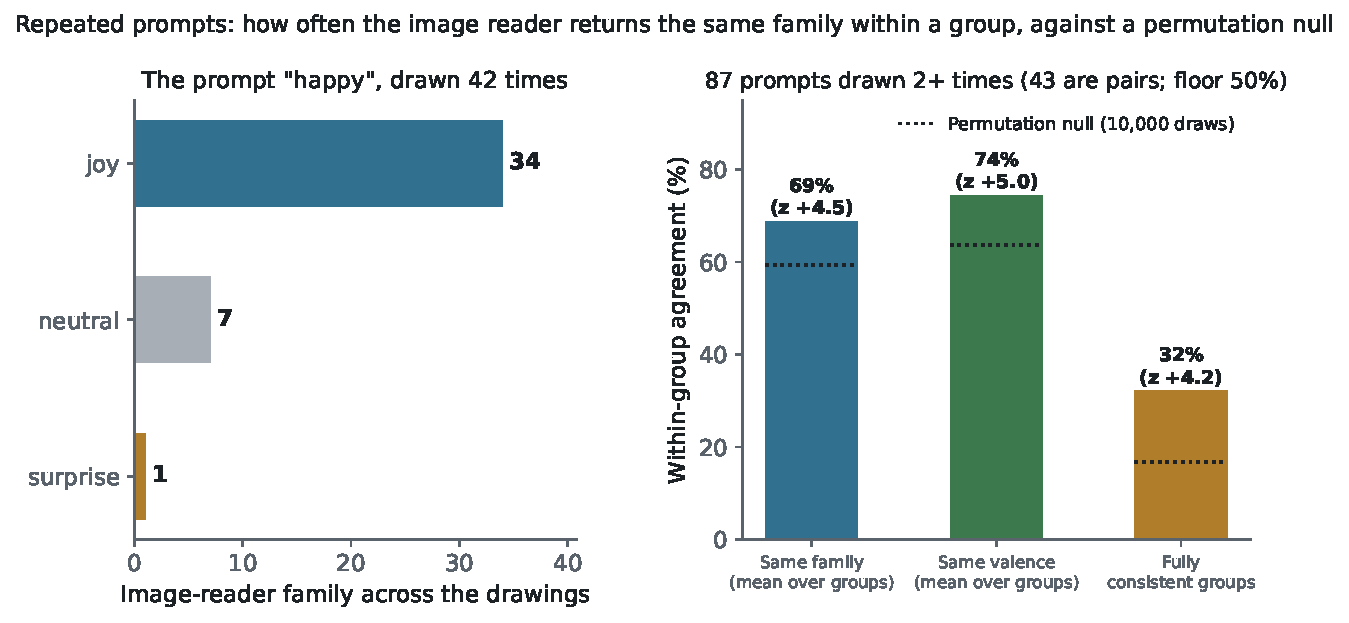
\includegraphics[width=0.98\textwidth]{../figures/fig4_consistency.pdf}\end{center}
Given an \emph{identical} prompt, the image reader returns the same family for 68.8\% of drawings
within a group against a permutation null of 59.4\% ($z\!=\!+4.5$; valence 74.5\% vs 63.7\%); 28
of 87 groups are fully consistent against 14.5 by chance (these pool corpus-wide repeats --- same text
from different visitors and re-submissions --- with generation parameters unrecorded, so the figure
bounds the whole prompt$\rightarrow$image$\rightarrow$reader chain). Half the groups are pairs
(floor 50\%). ``happy'' \(\times\)42 produced 34 joy, 7 neutral, 1 surprise.

\subsection{Finding 4 --- describe-then-extract agrees far more closely}
\begin{center}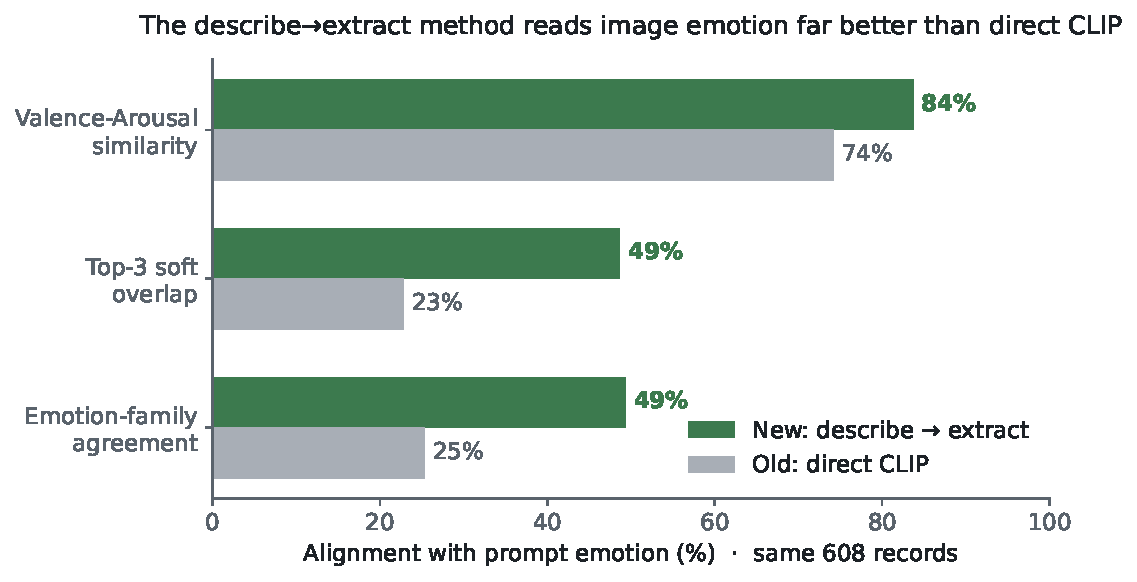
\includegraphics[width=0.9\textwidth]{../figures/fig2_method_comparison.pdf}\end{center}
Like for like (same GoEmotions prompt reader, same 607 emotional records, same measures),
describe$\rightarrow$extract reaches 53.0\% family agreement against 22.4\% for direct CLIP
($+30.6$\,pp [$+25.5$, $+35.6$], cluster-level $p < 0.0001$), 64.0\% vs 31.1\% on valence sign and
50.6\% vs 26.4\% on top-3 overlap --- support for the supervisor's proposed architecture. Neither
reader has ground truth: this ranks two image readers against a third model's labels. The earlier
49.3\% vs 25.3\% (608 records, NLI prompt side; overlap corrected from 15\% to 23\% after a
label-space audit) is the historical v1 record.

\subsection{Finding 5 --- the reading rests on one word (template ablation)}
\begin{center}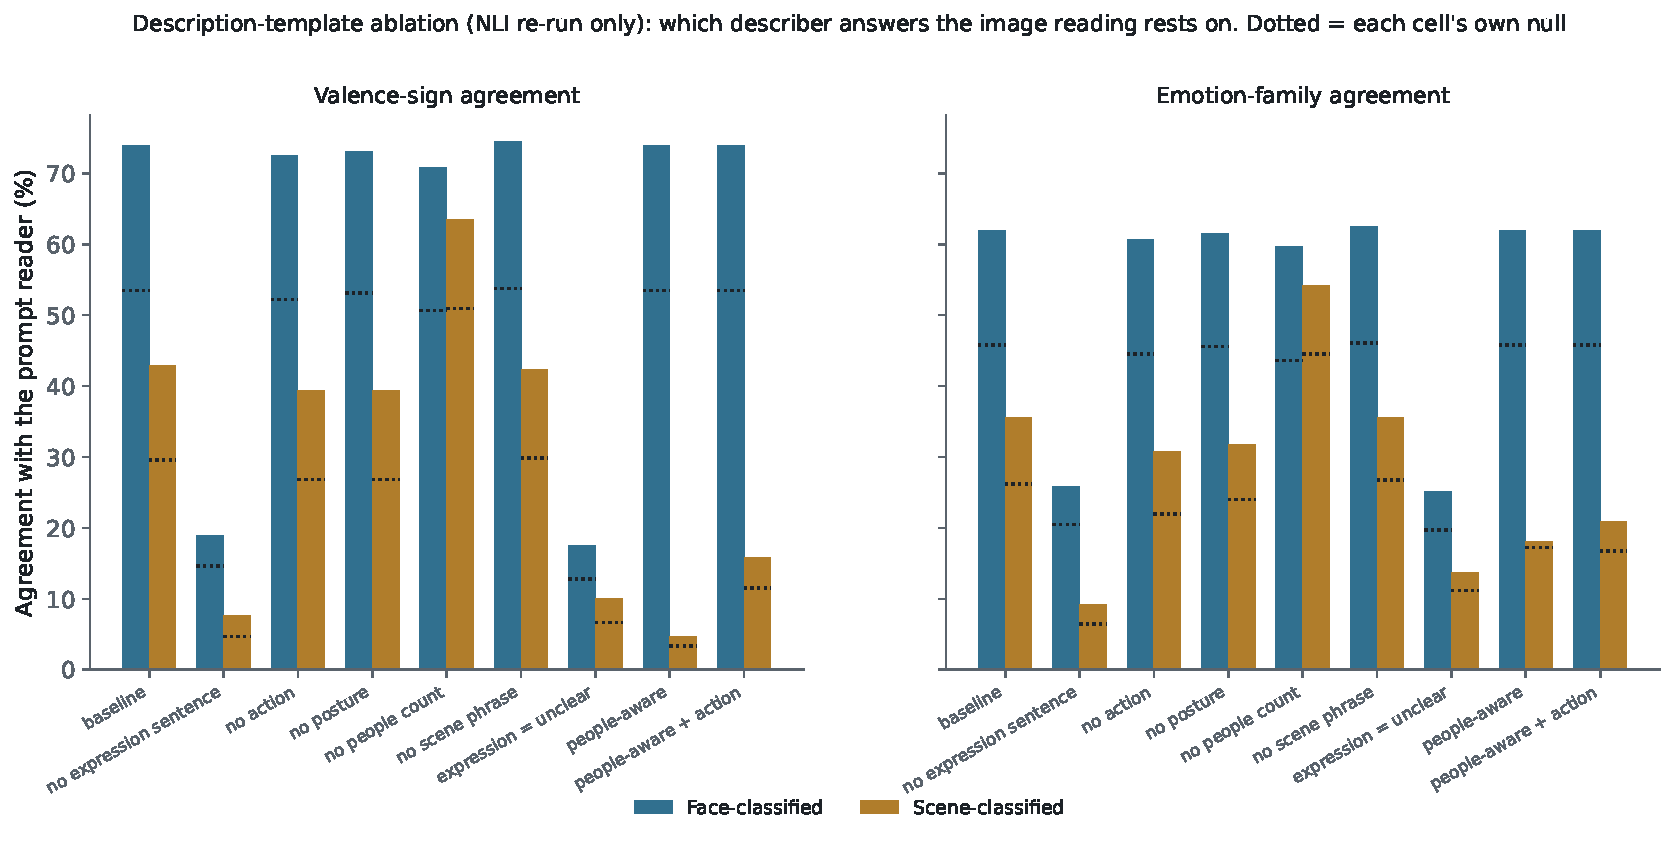
\includegraphics[width=0.98\textwidth]{../figures/fig8_ablation.pdf}\end{center}
Each record's five cached describer answers were re-composed under an altered template and only the
NLI stage re-run (\texttt{ablate\_nli.py}; a control re-run of the unmodified template reproduces
every baseline number exactly). Removing the expression sentence collapses all-emotional family
agreement from 53.0\% to 20.3\% (null 16.6\%, $z\!=\!+3.8$) and valence sign from 64.0\% to 15.3\%;
fixing the expression to ``unclear'' gives the same collapse; removing action, posture or scene
moves the rates by 1--3\,pp; removing the people count raises rates and nulls together (scene sign
63.5\% vs 50.9\%, $z\!=\!+5.0$). Under a \textbf{people-aware template} (``A drawing showing
\{scene\}.'' where no person is reported) the face rows are unchanged and \textbf{scene agreement
falls to its null}: valence sign 4.7\% vs 3.4\% ($z\!=\!+1.6$), family 18.0\% vs 17.3\% ($z\!=\!+0.6$).
The image reading rests on the describer's expression word (consistent with the 99.8\% copy rate);
the headline scene result was an artefact of an invented expression; the face/scene contrast is
faces, and only faces, for this reader; whether scene drawings hold a feeling a person can read is
what the human check tests.

\subsection{What is deliberately \emph{not} claimed}
\begin{itemize}
\item \textbf{``Positive emotions transfer better than negative''} --- retracted after re-audit: within a single-valence subset the sign/family null is degenerate ($z\!=\!0$) and the raw
gap is a base-rate artifact. The two automatic readers disagree in \emph{opposite} directions
(CLIP skews negative on line art; BLIP-VQA reports a smiling or happy expression for 57\% of
face-classified records and 66\% of all expression answers), so only the planned
\textbf{human-rating study} can adjudicate.
\item Fear, disgust and surprise are recovered at very low rates by both readers, on prompt-side
subsets of $n=16$ and $n=1$ and a surprise class largely composed of curiosity-mapped prompts; claims
are restricted to overall agreement and the face/scene contrast, and no directional valence claim is
made.
\end{itemize}

% ---------------- verification ----------------
\section{Verification and robustness}
\begin{itemize}
\item \textbf{Null baselines everywhere.} All metrics referenced to 300 random pairings; every rate
carries a clustered-bootstrap 95\% interval; degenerate nulls are detected automatically and carry no $z$.
\item \textbf{Re-audit (1 and 9 September 2026).} The analysis was re-derived twice; the corrections
(degenerate nulls, missing per-metric baselines, an overstated scene claim, undisclosed duplicates,
a consistency figure quoted without its null, a comparison that was not like for like, hand-typed
figures) were all applied and are listed below.
\item \textbf{Deduplication.} 249 duplicate-prompt records disclosed; every headline re-run on 763
distinct prompts --- face finding robust, scene finding weakened.
\item \textbf{Data integrity.} 1{,}025 unique ids, all image paths verified, all emotion fields
well-formed, no unhandled errors.
\item \textbf{Automated self-test} (\texttt{test.sh} + \texttt{test\_numeric.py}): environment,
data, redaction audit, analyses, live pipeline, pinned numeric values, figures --- \pass.
\end{itemize}

% ---------------- audit ----------------
\section{Final audit}
A six-dimension audit (code correctness; claim reproduction; document consistency; reproducibility;
legacy-code health; deep data integrity) was run as the final step, and \textbf{every finding was fixed
and re-verified}. The material findings and their resolutions:

\begin{center}
\begin{tabular}{@{}p{6.9cm}p{7.3cm}@{}}
\toprule
\textbf{Finding (severity)} & \textbf{Resolution}\\
\midrule
Label-space mismatch deflated the old method's top-3 overlap: 15\% $\rightarrow$ true 23\% (\textcolor{red}{major}) & Canonicalised \texttt{happiness}$\rightarrow$\texttt{joy}; ``tripled'' corrected to ``roughly doubled'' in every document. The conclusion that describe-then-extract agrees more closely is unchanged.\\
Two scripts silently included the 13 pre-test records (\textcolor{red}{major}) & Pre-test filter added; affected table now $n=984$ (values shift $\le$0.4pp; no finding changes).\\
README and four dashboards presented the superseded direct-CLIP era as current (\textcolor{red}{critical/major}) & README rewritten around the final architecture; stale dashboards and write-ups moved to \texttt{outputs/archive/} with visible supersession banners.\\
Face rule missed multi-word answers (``man is smiling'') --- $\sim$2.5\% leakage (minor) & Token-intersection matching; split refreshed (591/421), findings re-verified.\\
No pinned dependencies; setup script bypassed the venv; figures module missing from it (\textcolor{red}{major}) & \texttt{requirements.txt} (55 pinned packages); \texttt{setup.sh} now creates the venv and installs from it; figure generation added to the test suite.\\
Fragile old-baseline dependency (a legacy command would overwrite it) (\textcolor{red}{major}) & Baseline frozen as \texttt{results\_clip\_v2\_baseline.json}; comparison script points at the frozen copy.\\
``Repeated-prompt runs'' phrasing conflated corpus-wide repeats with consecutive runs (minor) & Reworded throughout; the pooling is now stated explicitly alongside the stricter consecutive-run count.\\
Assorted: two case-mismatched image paths (Linux-portability), unnormalised cached family scores, stale-cache crash path, misleading comments (minor) & All fixed; per-record paths verified against the on-disk listing; cache normalised and guarded.\\
\bottomrule
\end{tabular}
\end{center}

The audit also \emph{confirmed}: every published number reproduces exactly on a fresh run
(deterministic, seeded); the null/z machinery is statistically sound; the data chain is airtight
(1{,}025 unique ids, all paths resolve, zero malformed records); and the legacy baseline still runs.

\textbf{Second audit (9 September 2026)} against the marking criteria, with the resolutions:
the consistency null was quoted from no script (now computed in \texttt{data\_audit\_consistency.py},
59.4\%, $z{+}4.5$); the method comparison was not like for like (re-run in
\texttt{method\_comparison.py} with a paired, clustered test); no confidence intervals or kappa
(\texttt{inference.py}); degenerate nulls flagged by hand (now detected from the null's spread);
figures typed by hand (now generated from \texttt{analysis\_final.json} and its siblings); no numeric
tests (\texttt{test\_numeric.py}); metric code duplicated across scripts (one definition in
\texttt{emoviz/metrics.py}); the control set and the describer never audited (\texttt{audits.py});
no qualitative account of disagreements (\texttt{error\_taxonomy.py}); the description template never
ablated (\texttt{ablate\_nli.py}); no human anchor (\texttt{human\_check.py}, coding pending).

% ---------------- limitations ----------------
\section{Limitations and next steps}
\begin{itemize}
\item \textbf{Reader bias is the binding limitation.} BLIP-VQA's positivity bias and CLIP's negativity
bias bound what automatic measures can claim; the \textbf{human-rating study} is the designed
adjudicator, and a 120-drawing blind single-coder check has been set up as its first step.
\item Valence--arousal uses emotion-label centroids; a continuous lexicon (NRC-VAD) is a ready upgrade.
\item The face/scene rule is description-derived, and the template asserts an expression for drawings
with no person; the people-aware ablation shows the scene reading sits at chance without that clause,
so a scene-capable describer and a dedicated face detector are the next steps.
\item Hardware bounded model choice (sub-1B describers); results are nonetheless statistically strong.
\end{itemize}

% ---------------- repo map ----------------
\section{Repository guide}
\begin{center}
\begin{tabular}{@{}p{5.6cm}p{8.6cm}@{}}
\toprule
\textbf{File} & \textbf{Role}\\
\midrule
\texttt{describe\_extract.py} & The pipeline (crash-safe, resumable)\\
\texttt{analysis\_final.py} & Final analysis: splits, similarity ladder, nulls, dedup\\
\texttt{data\_audit\_consistency.py} & Data accounting + repeated-prompt consistency\\
\texttt{similarity\_v2.py} & Old-vs-new method comparison\\
\texttt{make\_figures.py} & All report figures, generated from the result files\\
\texttt{test.sh} + \texttt{test\_numeric.py} & Automated self-test: smoke layer plus pinned numeric values\\
\texttt{emoviz/metrics.py} & The one definition of every measure, split and null\\
\texttt{significance.py}, \texttt{inference.py} & Clustered test of the face/scene difference; CIs, kappa, Holm\\
\texttt{method\_comparison.py} & Like-for-like image-reader comparison with a paired test\\
\texttt{audits.py}, \texttt{error\_taxonomy.py} & Control and describer audits; failure-mode census\\
\texttt{ablate\_nli.py}, \texttt{human\_check.py} & Description-template ablation; blind single-coder check\\
\texttt{emoviz/} & Core package (loader; earlier baseline reader)\\
\texttt{outputs/RESULTS\_final.md} & Verified findings write-up\\
\texttt{outputs/describe\_extract.jsonl} & Full per-record pipeline output (1{,}025)\\
\texttt{outputs/analysis\_final.csv} & Per-record analysis table (1{,}012)\\
\texttt{outputs/analysis\_final.json} & Every reported number, machine-readable\\
\texttt{PIPELINE\_DESIGN.md} & Architecture options \& decisions\\
\bottomrule
\end{tabular}
\end{center}

\vspace{8pt}
\hrule
\vspace{6pt}
{\small\color{soft} Prepared as technical documentation for the dissertation project. All numbers
trace to re-runnable scripts in the repository; every figure regenerates from
\texttt{make\_figures.py}.}

\end{document}
